\documentclass[reqno,11pt]{amsart}

\usepackage{amsmath,amssymb,amsthm,mathtools}
\usepackage[top=2.6cm,bottom=2.6cm,left=2.9cm,right=2.9cm]{geometry}
\usepackage{xcolor}
\usepackage{tikz}
\usepackage{tikz-3dplot}
\usetikzlibrary{arrows.meta,calc,3d,shadings,positioning}
\usepackage{booktabs}
\usepackage{caption}
\captionsetup{font=small,labelfont=bf}
\usepackage[colorlinks=true,linkcolor=blue!60!black,citecolor=blue!60!black,urlcolor=blue!60!black]{hyperref}
\hypersetup{pdftitle={Torsion D-Brane Charges from H-Flux on Calabi-Yau Threefolds},pdfauthor={Deep Bhattacharjee, Ushashi Bhattacharya}}
\usepackage{doi}
\emergencystretch=2em
\raggedbottom

\newtheorem{theorem}{Theorem}[section]
\newtheorem{proposition}[theorem]{Proposition}
\newtheorem{lemma}[theorem]{Lemma}
\newtheorem{corollary}[theorem]{Corollary}
\theoremstyle{definition}
\newtheorem{definition}[theorem]{Definition}
\newtheorem{remark}[theorem]{Remark}
\newtheorem{example}[theorem]{Example}

\newcommand{\ZZ}{\mathbb{Z}}
\newcommand{\QQ}{\mathbb{Q}}
\newcommand{\RR}{\mathbb{R}}
\newcommand{\CC}{\mathbb{C}}
\newcommand{\KK}{K\!K}
\newcommand{\ch}{\operatorname{ch}}
\newcommand{\Td}{\operatorname{Td}}
\newcommand{\Ahat}{\widehat{A}}
\newcommand{\Sq}{\operatorname{Sq}}
\newcommand{\rk}{\operatorname{rank}}
\newcommand{\Zm}{\ZZ/m}
\DeclareMathOperator{\coker}{coker}
\DeclareMathOperator{\im}{im}
\DeclareMathOperator{\Tor}{Tor}
\DeclareMathOperator{\Hom}{Hom}
\DeclareMathOperator{\Ext}{Ext}

\title[Torsion D-brane charges from $H$-flux]{Torsion D-Brane Charges from $H$-Flux on Calabi--Yau Threefolds}

\author[D.~Bhattacharjee]{Deep Bhattacharjee}
\address{Electro-Gravitational Space Propulsion Laboratory (EGSPL), Bhubaneswar, Odisha 751030, India; formerly, University of Calcutta (Heramba Chandra College), 23/49 Gariahat Road, Golpark, Kolkata 700029, West Bengal, India}
\email{d.bhattacharjee@erl-forschung.de}
\email{itsdeep@live.com}
\email{egspl@proton.me}
\urladdr{https://orcid.org/0000-0003-0466-750X}

\author[U.~Bhattacharya]{Ushashi Bhattacharya}
\address{National Taiwan University, Taipei, Taiwan}
\email{rai.bhattacharya.in@gmail.com}
\urladdr{https://orcid.org/0009-0002-2254-3914}

\thanks{Corresponding author: Deep Bhattacharjee (\texttt{d.bhattacharjee@erl-forschung.de}); \texttt{egspl@proton.me} for matters concerning the code repository.}
\thanks{The expository parts of Sections~\ref{sec:ktheory}, \ref{sec:twisted} and~\ref{sec:index} revise the treatment of D.~Bhattacharjee, S.\,S.~Roy, R.~Sadhu and A.\,K.~Behera, \emph{KK theory and K theory for Type II strings formalism}, Asian Res.\ J.\ Math.\ \textbf{19} (2023), no.~9, 79--94, \doi{10.9734/arjom/2023/v19i9701}, and correct several statements made there. The main result, Theorem~\ref{thm:six}, gives an explicit presentation of the torsion and determines the even group as an abstract group by combining the twisted spectral sequence with twisted Poincar\'e duality and the universal coefficient theorem; the degeneration of the spectral sequence on a simply connected six-manifold was observed by Collinucci and Evslin \cite{CE07}, and the untwisted groups of Calabi--Yau threefolds are due to Doran and Morgan \cite{DM07}. The three-dimensional computation of Theorem~\ref{thm:three} and the circle bundles of Proposition~\ref{prop:tdualcheck} are consistency checks against established results: the circle-bundle groups and their exchange under T-duality are in Bouwknegt, Evslin and Mathai \cite[Section~4.2]{BEM04a}.}

\subjclass[2020]{19L50, 55N15, 55T25, 57R65, 81T30}
\keywords{Twisted K-theory, D-brane charge, Calabi--Yau threefold, T-duality}

\begin{document}

\begin{abstract}
Let $X$ be a connected closed spin$^c$ six-manifold with $H_1(X;\ZZ)=0$, for instance a simply connected Calabi--Yau threefold, and let $H\in H^3(X;\ZZ)$. We determine the twisted K-groups $K^{H,*}(X)$ as abstract groups: their torsion is the finite group $\Tor(H^3(X;\ZZ)/\ZZ H)$ in odd degree and its character group in even degree, and the ranks are $b_3-2$ and $2b_2$ for a flux of infinite order. When the cohomology is torsion-free and $H$ is $m$ times a primitive class this reads $K^{H,0}\cong\ZZ^{2b_2}\oplus\ZZ/m$, $K^{H,1}\cong\ZZ^{b_3-2}\oplus\ZZ/m$. When $H^3$ has torsion the torsion component of the flux changes the invariant factors, and we construct spin six-manifolds on which this happens. The same method gives the twisted K-groups of every closed oriented three-manifold, which are checked against T-duality for circle bundles over surfaces.
\end{abstract}

\maketitle

\section{Introduction}\label{sec:intro}

Ramond--Ramond charges of D-branes in Type II string theory on a compact space $X$ are classified by the topological K-theory of $X$ \cite{MM97,Wit98}, and in the presence of a Neveu--Schwarz three-form flux with integral class $H\in H^3(X;\ZZ)$ by the twisted K-theory $K^{H,*}(X)$ \cite{Wit98,BM00,Kap00}. The twisted groups are rarely written down for the spaces that matter most in compactification, the Calabi--Yau threefolds. This paper computes them.

\begin{theorem}\label{thm:six}
Let $X$ be a connected closed spin$^c$ six-manifold with $H_1(X;\ZZ)=0$ and Betti numbers $b_2=b_4$ and $b_3$, and let $H\in H^3(X;\ZZ)$. Put
\[
C_H=\Tor\bigl(H^3(X;\ZZ)/\ZZ H\bigr),\qquad C_H^\vee=\Hom(C_H,\QQ/\ZZ),
\]
and $\delta_H=1$ if $H$ has infinite order, $\delta_H=0$ if $H$ is torsion (including $H=0$).
Then, as abstract abelian groups,
\[
K^{H,0}(X)\;\cong\;\ZZ^{2+2b_2-2\delta_H}\oplus C_H^\vee,\qquad
K^{H,1}(X)\;\cong\;\ZZ^{b_3-2\delta_H}\oplus C_H ,
\]
and more precisely $K^{H,1}(X)\cong\ker\bigl(H\cup(-)\colon H^3(X;\ZZ)\to H^6(X;\ZZ)\bigr)/\ZZ H$. If $H^*(X;\ZZ)$ is torsion-free and $H=mH_0\neq0$ with $H_0$ primitive and $m\ge1$, then $C_H\cong\ZZ/m$,
\[
K^{H,0}(X)\;\cong\;\ZZ^{2b_2}\oplus\ZZ/m,\qquad
K^{H,1}(X)\;\cong\;\ZZ^{b_3-2}\oplus\ZZ/m ,
\]
and $K^{H,0}(X)\cong H^2(X;\ZZ)\oplus H^4(X;\ZZ)\oplus H^6(X;\ZZ)/mH^6(X;\ZZ)$, $K^{H,1}(X)\cong H_0^{\perp}/\ZZ H$, where $H_0^\perp\subset H^3(X;\ZZ)$ is the kernel of $y\mapsto\langle H_0\cup y,[X]\rangle$; in this case the spin$^c$ hypothesis is not needed.
\end{theorem}

For $H=0$ the untwisted groups are $K^0(X)\cong\ZZ^{2+2b_2}\oplus T^\vee$ and $K^1(X)\cong\ZZ^{b_3}\oplus T$ with $T=\Tor H^3(X;\ZZ)$, which for a Calabi--Yau threefold agrees with Doran and Morgan \cite{DM07}. In the torsion-free case, switching on a flux of divisibility $m$ removes two free generators from each parity and replaces them by a cyclic group of order $m$ in each parity. In Type IIA the two lost even classes are the point class and the fundamental class, the charges of a D0-brane and of a D6-brane filling $X$; the D0-brane survives as a charge of order $m$. In Type IIB the lost odd classes are $H$ itself and a class dual to it; the D3-branes that survive are those wrapping three-cycles $W$ with $\int_W H=0$, which is the Freed--Witten condition \cite{FW99}, and the D3-brane on the cycle Poincar\'e dual to $H_0$ carries a charge of order $m$. Every simply connected Calabi--Yau threefold with torsion-free cohomology satisfies the hypotheses, so the theorem gives, for the quintic threefold with $b_2=1$, $b_3=204$,
\[
K^{H,0}\cong\ZZ^2\oplus\ZZ/m,\qquad K^{H,1}\cong\ZZ^{202}\oplus\ZZ/m .
\]
When $H^3(X;\ZZ)$ has torsion the group $C_H$ depends on more than the divisibility of the free part of $H$: on the spin six-manifolds $X_n$ of Proposition~\ref{prop:surgery}, with $H^3(X_n;\ZZ)\cong\ZZ^2\oplus\ZZ/n$, the two fluxes $2a$ and $2a+c$ ($a$ primitive, $c$ of order $2$, $n=2$) give $C_H\cong\ZZ/2\oplus\ZZ/2$ and $C_H\cong\ZZ/4$ respectively (Corollary~\ref{cor:realized}).

The proof uses the Atiyah--Hirzebruch spectral sequence of twisted K-theory, whose first differential is $d_3=\Sq^3_\ZZ-H\cup(-)$ by the theorem of Atiyah and Segal \cite{AS06}. On a six-manifold with $H_1=0$ every other differential vanishes for reasons of degree and the integral Steenrod operation $\Sq^3_\ZZ$ contributes nothing, as Collinucci and Evslin observed \cite{CE07}; the torsion is produced by the cup product with $H$ on $H^3$, which through Poincar\'e duality is a unimodular alternating form on the free part of $H^3$, and a lattice argument (Lemma~\ref{lem:lattice}) identifies its cokernel and the quotient of its kernel. The odd group has a single filtration quotient and is read off directly. The even group is an iterated extension which need not split when $H^3$ has torsion; we do not resolve the extension but determine the group by Poincar\'e duality in twisted K-theory (Tu \cite{Tu09}) and the universal coefficient theorem of Rosenberg and Schochet \cite{RS87}, which identify its torsion with the character group of the torsion of the odd group for the opposite twist.

The same argument applies to three-manifolds, where the cup product with $H$ only acts on $H^0$.

\begin{theorem}\label{thm:three}
Let $M$ be a connected closed oriented three-manifold and let $H=k\,[M]^\vee\in H^3(M;\ZZ)\cong\ZZ$ with $k\neq0$. Then
\[
K^{H,0}(M)\cong H^2(M;\ZZ),\qquad K^{H,1}(M)\cong H^1(M;\ZZ)\oplus\ZZ/k .
\]
\end{theorem}

For $M=S^3$ this is the classical result $K^{H,0}(S^3)=0$, $K^{H,1}(S^3)=\ZZ/k$ behind the $\ZZ/k$-valued D0-charge of \cite{MMS01}. For circle bundles over a closed surface Theorem~\ref{thm:three} can be tested against T-duality: by Bouwknegt, Evslin and Mathai \cite{BEM04a,BEM04b} the circle bundle of Euler number $e$ with $k$ units of flux is T-dual to the circle bundle of Euler number $k$ with $e$ units of flux, and T-duality shifts the degree of twisted K-theory by one. Proposition~\ref{prop:tdualcheck} verifies that the groups of Theorem~\ref{thm:three} satisfy this exchange for every genus and every pair $(e,k)$, torsion included; the four cases and their exchange are those of \cite[Section~4.2]{BEM04a}, so this is a check of Theorem~\ref{thm:three} against a known computation, not a new result.

The remaining sections set up the K-theory, the twisted K-theory, the index theory and the Chern character needed for the statements above, in a form that corrects the earlier treatment cited in the title footnote: the definition of the odd K-group, the proof of Bott periodicity, the form of the Riemann--Roch formula for the push-forward, the data entering T-duality, and the integrality of Ramond--Ramond fields. Every finite computation in the paper (the groups of the examples, the Smith normal forms, the Riemann--Roch identities) is reproduced by a short Python script, see Appendix~\ref{app:code}.

\section{K-theory and the Atiyah--Hirzebruch spectral sequence}\label{sec:ktheory}

\subsection{K-groups}
Let $X$ be a compact Hausdorff space. $K^0(X)$ is the Grothendieck group of the monoid of isomorphism classes of complex vector bundles on $X$ under direct sum; for a pointed space $(X,x_0)$ the reduced group $\widetilde K^0(X)$ is the kernel of the restriction $K^0(X)\to K^0(x_0)=\ZZ$, and $K^0(X)\cong\widetilde K^0(X)\oplus\ZZ$. For connected $X$ the restriction to the base point is the rank, so $\widetilde K^0(X)$ is the kernel of the rank map $K^0(X)\to H^0(X;\ZZ)=\ZZ$; for a space with $c$ components the rank map has target $\ZZ^c$ and the two kernels differ, which is why the reduced group is defined through the base point. For a pointed space the reduced groups are extended to negative degrees by suspension,
\begin{equation}\label{eq:K1}
\widetilde K^{-n}(X)=\widetilde K^0(\Sigma^nX),\qquad K^{-n}(X)=\widetilde K^{-n}(X_+)=\widetilde K^0\bigl(\Sigma^n(X_+)\bigr),
\end{equation}
where $X_+$ is $X$ with a disjoint base point and $\Sigma$ the reduced suspension; for suspensions of surfaces of higher genus see also \cite{Bha22a}. In particular $K^{-1}(X)=\widetilde K^0(S^1\wedge X_+)$, which is also the K-theory with compact supports of $X\times\RR$.\footnote{The group $\widetilde K^0(\Sigma X)$, with $X$ itself as the pointed space, is the reduced group $\widetilde K^{-1}(X)$; for connected $X$ the two agree, $K^{-1}(X)\cong\widetilde K^{-1}(X)$, because $\Sigma(X_+)=\Sigma X\vee S^1$ and $\widetilde K^0(S^1)=0$. For a space with $c$ components the unreduced group has $c$ copies of $\widetilde K^{-1}(S^0)=0$ added, so the two agree there as well; the distinction matters in even degree, where $K^0(X)$ and $\widetilde K^0(X)$ differ by the rank. We write $K^1$ for $K^{-1}$ throughout, which is harmless by periodicity.}

\begin{theorem}[Bott periodicity \cite{Ati67}]\label{thm:bott}
The product with the Bott class $\beta\in\widetilde K^0(S^2)$ is an isomorphism $\widetilde K^{-n}(X)\to\widetilde K^{-n-2}(X)$ for every compact pointed $X$ and every $n\ge0$. Hence $\widetilde K^0(S^{2j})\cong\ZZ$, $\widetilde K^0(S^{2j+1})=0$, $\widetilde K^{1}(S^{2j+1})\cong\ZZ$ and $\widetilde K^{1}(S^{2j})=0$.
\end{theorem}

In the language of $C^*$-algebras the statement is that the Bott element $\beta\in\KK(\CC,C_0(\RR^2))$ is invertible, so that $C_0(\RR^2)$ is $\KK$-equivalent to $\CC$ and $K_*(A\otimes C_0(\RR^2))\cong K_*(A)$ for every $C^*$-algebra $A$. It is not an isomorphism of algebras: $C_0(\RR^2)\otimes\mathcal K$ has the nontrivial ideals $C_0(U)\otimes\mathcal K$ for open $U\subset\RR^2$, whereas $\mathcal K$ is simple, so $C(X)\otimes C_0(\RR^2)$ and $C(X)$ are never stably isomorphic. Periodicity is a statement about K-theory, and its proof \cite{Ati67} goes through the clutching construction or, in Kasparov's framework \cite{Kas81}, through the construction of an inverse to $\beta$.

\subsection{The spectral sequence}
For a finite CW complex $X$ the skeleton filtration gives the Atiyah--Hirzebruch spectral sequence \cite{AH61}
\begin{equation}\label{eq:ahss}
E_2^{p,q}=H^p\bigl(X;K^q(\mathrm{pt})\bigr)=\begin{cases}H^p(X;\ZZ)&q\text{ even},\\ 0&q\text{ odd},\end{cases}\qquad\Longrightarrow\qquad K^{p+q}(X).
\end{equation}
The differentials $d_r$ have bidegree $(r,1-r)$ and vanish for even $r$. The first one is the integral Steenrod operation
\begin{equation}\label{eq:d3}
d_3=\Sq^3_\ZZ=\beta\circ\Sq^2\circ\rho_2\colon H^p(X;\ZZ)\longrightarrow H^{p+3}(X;\ZZ),
\end{equation}
where $\rho_2$ is reduction modulo $2$ and $\beta$ the Bockstein of $0\to\ZZ\to\ZZ\to\ZZ/2\to0$; this is due to Atiyah and Hirzebruch \cite{AH61}. Two consequences are used below: $\Sq^3_\ZZ$ vanishes on $H^0$ and on $H^2$, because $\Sq^2$ vanishes on classes of degree less than two, while for an integral class $x$ of degree two $\Sq^2\rho_2x=(\rho_2x)^2=\rho_2(x^2)$ is the reduction of an integral class and so has zero Bockstein; and the image of $\Sq^3_\ZZ$ consists of torsion classes, because it factors through a Bockstein. The higher differentials $d_5,d_7,\dots$ are not given by primary cohomology operations and need not vanish in general; no claim about them is needed in this paper because they vanish for reasons of degree in all the cases considered.

The spectral sequence gives $K^*(X)$ only up to extensions: $K^n(X)$ carries the filtration $F^pK^n(X)=\ker\bigl(K^n(X)\to K^n(X^{(p-1)})\bigr)$ and $E_\infty^{p,n-p}=F^p/F^{p+1}$. When $E_\infty^{p,n-p}$ is free for all $p$ but the largest one, every extension splits and $K^n(X)\cong\bigoplus_pE_\infty^{p,n-p}$.

\begin{example}\label{ex:even}
If $H^*(X;\ZZ)$ is torsion-free and concentrated in even degrees then every differential has zero source or zero target, the filtration quotients are free, and $K^0(X)\cong\bigoplus_pH^{2p}(X;\ZZ)$, $K^1(X)=0$. This covers $S^{2j}$, $\CC P^n$ and K3 surfaces, whose cohomology is torsion-free and sits in degrees $0$, $2$, $4$ with ranks $1$, $22$, $1$ \cite[Chapter~VIII]{BHPV04} (for the involutions of K3 surfaces and their Enriques and Kummer quotients see also \cite{BRB22,BN26}): $K^0(K3)\cong\ZZ^{24}$ and $K^1(K3)=0$. For a torus the K\"unneth theorem gives $K^*(T^n)$ as the exterior algebra on $n$ odd generators, so $K^0(T^n)\cong K^1(T^n)\cong\ZZ^{2^{n-1}}$. For a Calabi--Yau threefold with torsion-free cohomology the untwisted groups are $K^0\cong\ZZ^{2+2h^{1,1}}$ and $K^1\cong\ZZ^{2+2h^{2,1}}$, see Proposition~\ref{prop:untwistedsix}. Table~\ref{tab:kgroups} collects these.
\end{example}

\begin{table}[ht]
\centering
\caption{Untwisted K-groups of some compactification spaces (Example~\ref{ex:even}; the Calabi--Yau line assumes torsion-free cohomology). The convention is that of particle charges in $\RR^{1,3}\times X$: a brane extended along the time direction only and wrapping $W\subset X$ has the charge $\iota_!E\in K^*(X)$ of Section~\ref{sec:index}; then Type IIA branes wrap even-dimensional cycles of $X$ and their charges lie in $K^0(X)$, Type IIB branes wrap odd-dimensional cycles and their charges lie in $K^1(X)$ \cite{Wit98}. For a brane filling $\RR^{1,3}$ the internal cycle has dimension $p-3$ and the parities are reversed.}
\label{tab:kgroups}
\begin{tabular}{lccc}
\toprule
$X$ & $\dim X$ & $K^0(X)$ & $K^1(X)$\\
\midrule
$S^2$ & 2 & $\ZZ^2$ & $0$\\
$S^4$ & 4 & $\ZZ^2$ & $0$\\
$\CC P^2$ & 4 & $\ZZ^3$ & $0$\\
$\CC P^3$ & 6 & $\ZZ^4$ & $0$\\
K3 & 4 & $\ZZ^{24}$ & $0$\\
$T^6$ & 6 & $\ZZ^{32}$ & $\ZZ^{32}$\\
Calabi--Yau threefold & 6 & $\ZZ^{2+2h^{1,1}}$ & $\ZZ^{2+2h^{2,1}}$\\
\bottomrule
\end{tabular}
\end{table}

\subsection{Kasparov's bivariant theory}
For separable $C^*$-algebras $A$ and $B$, Kasparov's group $\KK(A,B)=\KK_0(A,B)$ \cite{Kas81} is the set of homotopy classes of triples $(E,\phi,F)$ with $E$ a countably generated $\ZZ/2$-graded Hilbert $B$-module, $\phi\colon A\to\mathcal L(E)$ a $*$-homomorphism by even operators and $F\in\mathcal L(E)$ a bounded odd operator with $\phi(a)(F^2-1)$, $\phi(a)(F-F^*)$ and $[\phi(a),F]$ compact for all $a\in A$, so that $F$ is Fredholm modulo the compact operators on the support of $\phi$. The Kasparov product $\KK(A,B)\times\KK(B,C)\to\KK(A,C)$ makes these groups the morphisms of an additive category, and $K_0(B)=\KK(\CC,B)$, $K_1(B)=\KK(\CC,B\otimes C_0(\RR))$. For $B=C(X)$ this is $K^0(X)$ and $K^1(X)$. A brane--antibrane pair with Chan--Paton bundles $E_1,E_2$ and tachyon $T\colon E_1\to E_2$ defines the Kasparov module $(\Gamma(E_1)\oplus\Gamma(E_2),\,\phi,\,\bigl(\begin{smallmatrix}0&T^*\\T&0\end{smallmatrix}\bigr))$ with $A=\CC$ and $B=C(X)$: the sections form a Hilbert $C(X)$-module, $\Gamma(E_1)$ in even and $\Gamma(E_2)$ in odd degree, $\phi(\lambda)$ is the scalar multiplication by $\lambda\in\CC$, and the operator is bounded and odd, with $T^*T-1$ and $TT^*-1$ compact wherever $T$ is invertible up to compacts, so the triple is a cycle for $\KK(\CC,C(X))=K^0(X)$ and its class is $[E_1]-[E_2]$. If instead $\phi$ is taken to be the multiplication by functions, the same triple is a cycle for $\KK(C(X),C(X))$, which is a different group in general ($\KK(C(S^1),C(S^1))\cong\ZZ^2$ while $K^0(S^1)\cong\ZZ$); the charge class is recovered from it by restricting the first argument along the unit $\CC\to C(X)$. This is the K-theoretic form of Sen's descent relations and of the brane--antibrane tachyon condensation \cite{Sen98,Sen98b,Wit98}.

\section{Twisted K-theory}\label{sec:twisted}

\subsection{Definition}
Let $X$ be a finite CW complex, for instance a compact manifold, and $H\in H^3(X;\ZZ)$. Since $H^3(X;\ZZ)=[X,K(\ZZ,3)]=[X,B\,PU(\mathcal H)]$ for a separable infinite-dimensional Hilbert space $\mathcal H$, the class $H$ determines, up to isomorphism, a locally trivial bundle $\mathcal K_H\to X$ with fibre the compact operators $\mathcal K(\mathcal H)$ and structure group $PU(\mathcal H)$. Its algebra of sections $A_H=\Gamma(X,\mathcal K_H)$ is a continuous-trace $C^*$-algebra with spectrum $X$ and Dixmier--Douady class $H$ \cite{Ros89}, and
\begin{equation}\label{eq:twistedK}
K^{H,n}(X):=K_{-n}(A_H),\qquad n\in\ZZ/2 .
\end{equation}
For $H=0$ this is $K^{-n}(X)$. For torsion $H$ the same groups are obtained from a bundle of finite-dimensional matrix algebras, the Azumaya algebra of Donovan and Karoubi \cite{DK70}; a class of infinite order is not represented by a finite-dimensional bundle, since the Dixmier--Douady class of a bundle of $n\times n$ matrix algebras is $n$-torsion, and the compact-operator model is needed. The groups $K^{H,*}(X)$ are modules over $K^0(X)$, are functorial in pairs $(X,H)$, and depend only on the class $H$ up to the action of $H^2(X;\ZZ)$ on the choice of bundle \cite{AS04}.

\subsection{The twisted spectral sequence}
The skeleton filtration of $X$ gives a spectral sequence with the same $E_2$ term \eqref{eq:ahss} converging to $K^{H,*}(X)$ \cite{Ros89,AS06}. Its first differential is no longer a cohomology operation alone.

\begin{theorem}[Atiyah--Segal \cite{AS06}]\label{thm:twistedd3}
The differential $d_3$ of the spectral sequence of $K^{H,*}(X)$ is
\[
d_3=\Sq^3_\ZZ-H\cup(-)\colon H^p(X;\ZZ)\longrightarrow H^{p+3}(X;\ZZ).
\]
\end{theorem}

The sign of the second term depends on conventions and plays no role in what follows. Rationally the higher differentials are expressed through Massey products with $H$ \cite{AS06}; they are not primary operations and there is no universal formula of the form ``$d_5=$ a Steenrod operation twisted by $H$''. In the two situations treated in this paper the higher differentials vanish because their sources or targets are zero, so Theorem~\ref{thm:twistedd3} determines the associated graded groups; the extension and duality arguments of Sections~\ref{sec:six} and~\ref{sec:three} then determine the abstract groups.

\begin{figure}[ht]
\centering
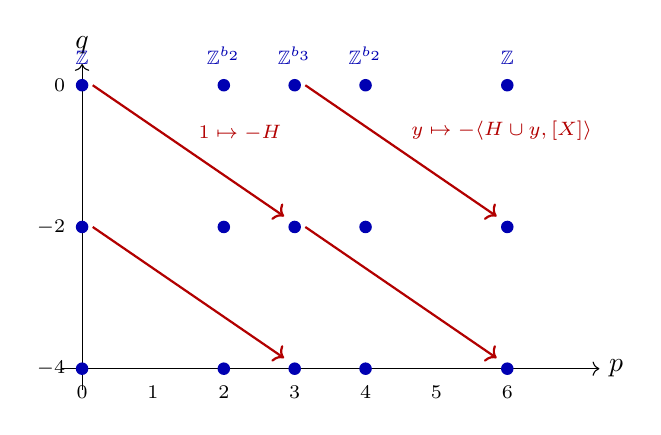
\begin{tikzpicture}[scale=0.9]
\draw[->] (-0.3,0) -- (7.3,0) node[right] {$p$};
\draw[->] (0,-0.3) -- (0,4.3) node[above] {$q$};
\foreach \p in {0,...,6} \node[below,font=\scriptsize] at (\p,-0.1) {\p};
\foreach \q/\l in {0/-4,2/-2,4/0} \node[left,font=\scriptsize] at (-0.1,\q) {$\l$};
\foreach \q in {0,2,4}{
  \node[circle,fill=blue!70!black,inner sep=1.6pt] at (0,\q) {};
  \node[circle,fill=blue!70!black,inner sep=1.6pt] at (2,\q) {};
  \node[circle,fill=blue!70!black,inner sep=1.6pt] at (3,\q) {};
  \node[circle,fill=blue!70!black,inner sep=1.6pt] at (4,\q) {};
  \node[circle,fill=blue!70!black,inner sep=1.6pt] at (6,\q) {};
}
\node[font=\scriptsize,blue!70!black,above] at (0,4.15) {$\ZZ$};
\node[font=\scriptsize,blue!70!black,above] at (2,4.15) {$\ZZ^{b_2}$};
\node[font=\scriptsize,blue!70!black,above] at (3,4.15) {$\ZZ^{b_3}$};
\node[font=\scriptsize,blue!70!black,above] at (4,4.15) {$\ZZ^{b_2}$};
\node[font=\scriptsize,blue!70!black,above] at (6,4.15) {$\ZZ$};
\draw[->,thick,red!70!black] (0.15,4) -- (2.85,2.15) node[midway,above right,font=\scriptsize] {$1\mapsto -H$};
\draw[->,thick,red!70!black] (3.15,4) -- (5.85,2.15) node[midway,above right,font=\scriptsize] {$y\mapsto -\langle H\cup y,[X]\rangle$};
\draw[->,thick,red!70!black] (0.15,2) -- (2.85,0.15);
\draw[->,thick,red!70!black] (3.15,2) -- (5.85,0.15);
\end{tikzpicture}
\caption{The $E_2$ page of the twisted Atiyah--Hirzebruch spectral sequence of a six-manifold with $H_1=0$ and torsion-free cohomology ($d_r$ has bidegree $(r,1-r)$). The columns $p=1$ and $p=5$ are empty. The only differentials that can be nonzero are the two $d_3$ shown, the cup product with $H$ from $H^0$ to $H^3$ and from $H^3$ to $H^6$; every later page coincides with $E_4$. With torsion in $H^3$ and $H^4$ the picture is the same, with $\ZZ^{b_3}$ and $\ZZ^{b_2}$ in columns $3$ and $4$ replaced by $\ZZ^{b_3}\oplus T$ and $\ZZ^{b_2}\oplus T$.}
\label{fig:ahss}
\end{figure}

\section{Six-manifolds and Calabi--Yau threefolds}\label{sec:six}

Throughout this section $X$ is a connected closed six-manifold with $H_1(X;\ZZ)=0$; simple connectivity implies this and is not needed. For the duality step, Lemma~\ref{lem:duality}, $X$ is also spin$^c$; a Calabi--Yau threefold is spin, hence spin$^c$. We write $T=\Tor H^3(X;\ZZ)$ and $L=H^3(X;\ZZ)/T$.

\begin{lemma}\label{lem:cohomology}
$H^0\cong H^6\cong\ZZ$, $H^1=H^5=0$, $H^2\cong\ZZ^{b_2}$ is free, $H^3\cong\ZZ^{b_3}\oplus T$ with $T\cong\Tor H_2(X;\ZZ)$, and $H^4\cong\ZZ^{b_2}\oplus T$. The cup product pairing
\begin{equation}\label{eq:omega}
\omega\colon L\times L\to\ZZ,\qquad\omega(y,z)=\langle y\cup z,[X]\rangle,
\end{equation}
is well defined, unimodular and alternating.
\end{lemma}

\begin{proof}
By the universal coefficient theorem $H^1\cong\Hom(H_1,\ZZ)=0$, $H^2\cong\Hom(H_2,\ZZ)\oplus\Ext(H_1,\ZZ)=\Hom(H_2,\ZZ)$ is free, and $\Tor H^3\cong\Ext(H_2,\ZZ)\cong\Tor H_2$. Poincar\'e duality gives $H^5\cong H_1=0$ and $H^4\cong H_2$, whose torsion is $T$. The pairing $H^3\times H^3\to\ZZ$ kills torsion, so descends to $L$; it is skew because $y\cup z=-z\cup y$ in odd degree, alternating because $2\,y\cup y=0$ and $H^6$ is torsion-free, and unimodular because Poincar\'e duality and the universal coefficient theorem identify $L$ with $\Hom(H_3,\ZZ)\cong\Hom(L,\ZZ)$ through it.
\end{proof}

\begin{proposition}\label{prop:untwistedsix}
If $H^*(X;\ZZ)$ is torsion-free then $K^0(X)\cong H^0\oplus H^2\oplus H^4\oplus H^6\cong\ZZ^{2+2b_2}$ and $K^1(X)\cong H^3(X;\ZZ)\cong\ZZ^{b_3}$. For a Calabi--Yau threefold, torsion included, $\widetilde K^0(X)\cong H^2\oplus H^4\oplus 2H^6$ and $K^1(X)\cong H^1\oplus H^3\oplus H^5$ by Doran and Morgan \cite{DM07}.
\end{proposition}

\begin{proof}
In \eqref{eq:ahss} the differential $d_3=\Sq^3_\ZZ$ vanishes on $H^0$ and $H^2$ by the remarks after \eqref{eq:d3}, and on $H^3$ it lands in the torsion of $H^6\cong\ZZ$, so it vanishes there too; $H^1=H^5=0$ removes the remaining sources and targets. The differentials $d_5\colon E^{p}\to E^{p+5}$ and $d_7\colon E^p\to E^{p+7}$ have zero source or target for every $p$ between $0$ and $6$ except $d_5\colon E^{0}\to E^{5}=0$ and $d_5\colon E^1=0\to E^6$. So $E_2=E_\infty$, every filtration quotient is free and the extensions split. The second statement is proved in \cite{DM07} through the Postnikov tower of $BSU$; its torsion agrees with the untwisted case of Theorem~\ref{thm:six} below.
\end{proof}

\begin{lemma}\label{lem:lattice}
Let $L$ be a free abelian group of finite rank with a unimodular alternating form $\omega$, let $H_0\in L$ be primitive and $H=mH_0$ with $m\ge1$. Then the homomorphism $\omega(H,-)\colon L\to\ZZ$ has image $m\ZZ$, its kernel $H_0^\perp$ is a direct summand of $L$ of corank one containing $H_0$, and
\[
H_0^\perp/\ZZ H\;\cong\;\ZZ^{\rk L-2}\oplus\ZZ/m .
\]
\end{lemma}

\begin{proof}
Unimodularity means that $y\mapsto\omega(y,-)$ is an isomorphism $L\to\operatorname{Hom}(L,\ZZ)$, so it carries the primitive vector $H_0$ to a primitive functional, which takes the value $1$ somewhere; hence $\omega(H_0,-)$ is onto $\ZZ$ and $\omega(H,-)=m\,\omega(H_0,-)$ has image $m\ZZ$. The kernel $H_0^\perp$ of a surjection onto $\ZZ$ is a direct summand of corank one, and $H_0\in H_0^\perp$ because $\omega$ is alternating. A primitive vector of $L$ lying in a direct summand is primitive in that summand, so $H_0^\perp=\ZZ H_0\oplus L'$ with $L'$ free of rank $\rk L-2$, and $H_0^\perp/\ZZ mH_0\cong\ZZ/m\oplus L'$.
\end{proof}

\subsection{The spectral sequence}
Let $H\in H^3(X;\ZZ)$ and let $f_H\colon H^3(X;\ZZ)\to\ZZ$, $f_H(y)=\langle H\cup y,[X]\rangle$; it kills $T$ and factors through $\omega(\bar H,-)$ on $L$, where $\bar H$ is the image of $H$ in $L$. Since $\omega$ is alternating, $f_H(H)=0$ and $\ZZ H\subset\ker f_H$.

\begin{lemma}\label{lem:degenerate}
In the spectral sequence of $K^{H,*}(X)$ the only differentials with nonzero source and target are
\[
d_3\colon H^0\to H^3,\ 1\mapsto -H,\qquad d_3\colon H^3\to H^6,\ y\mapsto-f_H(y)\,[X]^\vee,
\]
and $E_4=E_\infty$. Consequently
\[
E_\infty^{0}=\ker(1\mapsto H),\quad E_\infty^{2}=H^2,\quad E_\infty^{3}=\ker f_H/\ZZ H,\quad E_\infty^{4}=H^4,\quad E_\infty^{6}=\ZZ/\im f_H,
\]
$E_\infty^1=E_\infty^5=0$, where $E_r^{p}$ stands for $E_r^{p,q}$ with $q$ even.
\end{lemma}

\begin{proof}
By Theorem~\ref{thm:twistedd3}, $d_3=\Sq^3_\ZZ-H\cup(-)$. As in Proposition~\ref{prop:untwistedsix} the operation $\Sq^3_\ZZ$ vanishes on $H^0$ and $H^2$, its image on $H^3$ is torsion in $H^6\cong\ZZ$, and on $H^4$, $H^5$, $H^6$ its target is zero. The cup product with $H$ is zero from $H^1=0$, from $H^2$ to $H^5=0$ and from $H^4$ to $H^7=0$; this leaves the two maps displayed, and the second one is $-f_H$ by definition. The columns $1$, $5$ and $7$ are zero, so every $d_r$ with $r\ge5$, whose source and target are columns at distance $r$, has zero source or target ($(0,5)$, $(1,6)$, $(0,7)$ are the only pairs); hence $E_4=E_\infty$, for torsion twists as well as for twists of infinite order. The displayed groups are the $E_4$ terms.
\end{proof}

\begin{proposition}\label{prop:odd}
$K^{H,1}(X)\cong\ker f_H/\ZZ H$. This group has rank $b_3-2\delta_H$ and torsion subgroup $C_H=\Tor(H^3(X;\ZZ)/\ZZ H)$.
\end{proposition}

\begin{proof}
The odd group is filtered by the columns $1$, $3$ and $5$, of which only column $3$ is nonzero, so $K^{H,1}(X)=E_\infty^3=\ker f_H/\ZZ H$ and there is no extension problem. If $H$ is torsion then $f_H=0$, the quotient is $H^3/\ZZ H$, its rank is $b_3$ and its torsion is $C_H$ by definition. If $H$ has infinite order, write $\bar H=mH_0$ with $H_0\in L$ primitive. By Lemma~\ref{lem:lattice} the image of $f_H$ is $m\ZZ$ and $\ker f_H$ has rank $b_3-1$, so $\ker f_H/\ZZ H$ has rank $b_3-2$. The exact sequence $0\to\ker f_H/\ZZ H\to H^3/\ZZ H\to m\ZZ\to0$ has a free last term, so the torsion subgroups of its first two groups coincide, and the second one is $C_H$.
\end{proof}

\subsection{Duality determines the even torsion}
The even group $K^{H,0}(X)$ is an iterated extension of $E_\infty^{0}$, $H^2$, $H^4$ and $\ZZ/\im f_H$; when $T\ne0$ the extension by $H^4\cong\ZZ^{b_2}\oplus T$ need not split, and we determine the group by duality instead. Let $A_H=\Gamma(X,\mathcal K_H)$ be the continuous-trace algebra of Section~\ref{sec:twisted}, so that $K^{H,n}(X)=K_{-n}(A_H)$; its opposite algebra $A_H^{\mathrm{op}}$ is the continuous-trace algebra with Dixmier--Douady class $-H$.

\begin{lemma}\label{lem:duality}
For $X$ as above and spin$^c$,
\[
\Tor K^{H,0}(X)\;\cong\;\Hom\bigl(\Tor K^{-H,1}(X),\,\QQ/\ZZ\bigr).
\]
\end{lemma}

\begin{proof}
Tu's Poincar\'e duality for twisted K-theory \cite[Theorem~3.1]{Tu09} identifies the twisted K-theory of $X$ with twist $A_H$ with the twisted K-homology of $X$ with twist $C_\tau\hat\otimes A_H^{\mathrm{op}}$, where $C_\tau$ is the Clifford algebra bundle of the cotangent bundle. When $X$ is spin$^c$ the twist $C_\tau$ is trivial up to a degree shift by $\dim X=6$, which is even, so
\[
K_0(A_H)\;\cong\;\KK_0(A_{-H},\CC).
\]
The algebra $A_{-H}$ is separable, nuclear and belongs to the bootstrap class, being built from commutative algebras by finitely many extensions along the skeleta of $X$. The universal coefficient theorem of Rosenberg and Schochet \cite{RS87} therefore gives a short exact sequence
\[
0\longrightarrow\Ext^1_\ZZ\bigl(K_1(A_{-H}),\ZZ\bigr)\longrightarrow\KK_0(A_{-H},\CC)\longrightarrow\Hom\bigl(K_0(A_{-H}),\ZZ\bigr)\longrightarrow0 .
\]
The K-groups are finitely generated by Lemma~\ref{lem:degenerate}, so the last term is free and the first is finite; the first term is therefore the torsion subgroup of the middle one. Finally $K_1(A_{-H})=K^{-H,1}(X)$, and for a finitely generated group $G$ with torsion subgroup $G_{\mathrm{tor}}$ the sequence $0\to\ZZ\to\QQ\to\QQ/\ZZ\to0$ gives $\Ext^1_\ZZ(G,\ZZ)\cong\Hom(G_{\mathrm{tor}},\QQ/\ZZ)$.
\end{proof}

\begin{proof}[Proof of Theorem~\ref{thm:six}]
Proposition~\ref{prop:odd} is the odd statement. Since $\ZZ(-H)=\ZZ H$ and $f_{-H}=-f_H$, Proposition~\ref{prop:odd} for $-H$ gives $\Tor K^{-H,1}(X)\cong C_H$, and Lemma~\ref{lem:duality} gives $\Tor K^{H,0}(X)\cong C_H^\vee$. For the rank, tensor the filtration of Lemma~\ref{lem:degenerate} with $\QQ$: columns $2$ and $4$ contribute $b_2$ each; if $H$ has infinite order then $E^0_\infty=0$ and $E^6_\infty=\ZZ/m$ is finite, while if $H$ is torsion then $E^0_\infty\cong\ZZ$ (the kernel of $1\mapsto H$ is $k\ZZ$ for $H$ of order $k$, and $\ZZ$ for $H=0$) and $E^6_\infty=\ZZ$. This gives the rank $2+2b_2-2\delta_H$, and a finitely generated abelian group is the direct sum of its torsion subgroup and a free group.

In the torsion-free case $T=0$, $C_H=\Tor(L/\ZZ mH_0)\cong\ZZ/m$, and the extensions $0\to E_\infty^6\to F^4\to H^4\to0$ and $0\to F^4\to K^{H,0}(X)\to H^2\to0$ split because $H^4$ and $H^2$ are free, which gives $K^{H,0}(X)\cong H^2\oplus H^4\oplus H^6/mH^6$ without using Lemma~\ref{lem:duality}; and $K^{H,1}(X)\cong H_0^\perp/\ZZ H$ is Proposition~\ref{prop:odd} with Lemma~\ref{lem:lattice}.
\end{proof}

\subsection{The torsion group}
\begin{proposition}\label{prop:presentation}
Let $H$ have infinite order. Choose a splitting $H^3(X;\ZZ)\cong L\oplus T$ with $T\cong\bigoplus_{j=1}^r\ZZ/n_j$, and a basis of $L$ in which $\bar H=(m,0,\dots,0)$; write the component of $H$ in $T$ as $(t_1,\dots,t_r)$. Then $C_H$ is the abelian group with generators $u,c_1,\dots,c_r$ and relations
\begin{equation}\label{eq:presentation}
mu+\textstyle\sum_jt_jc_j=0,\qquad n_jc_j=0\quad(1\le j\le r),
\end{equation}
of order $m\,|T|$. In particular, if $T\cong\ZZ/n$ and the torsion component of $H$ is $t$, then with $g=\gcd(m,n,t)$
\[
C_H\;\cong\;\ZZ/g\oplus\ZZ/(mn/g),
\]
and the extension $0\to T\to C_H\to\ZZ/m\to0$ splits if and only if $\gcd(m,n)$ divides $t$.
\end{proposition}

\begin{proof}
The quotient $H^3/\ZZ H$ is the direct sum of the free group on the last $b_3-1$ basis vectors of $L$ and of the group generated by $u$ (the first basis vector) and the $c_j$ subject to \eqref{eq:presentation}; the latter is finite, of order the determinant $m\prod_jn_j$ of the relation matrix, so it is $C_H$. For $T=\ZZ/n$ the relation matrix $\bigl(\begin{smallmatrix}m&0\\t&n\end{smallmatrix}\bigr)$ has first determinantal divisor $g$ and determinant $mn$, so its Smith normal form is $\operatorname{diag}(g,mn/g)$. The map $C_H\to\ZZ/m$, $u\mapsto1$, $c\mapsto0$, has kernel the copy of $T$; a lift $u+sc$ of $1$ satisfies $m(u+sc)=(ms-t)c$, which vanishes for some $s$ exactly when $t\in mT$, that is when $\gcd(m,n)\mid t$. A change of the splitting replaces $t$ by $t+ms$ and $u$ by $u-sc$, which gives an equivalent presentation, so the group does not depend on the choices.
\end{proof}

For a torsion twist, $H\in T$, the group is simply $C_H=T/\langle H\rangle$, and Theorem~\ref{thm:six} reads $K^{H,1}(X)\cong\ZZ^{b_3}\oplus T/\langle H\rangle$, $K^{H,0}(X)\cong\ZZ^{2+2b_2}\oplus(T/\langle H\rangle)^\vee$; for $H=0$ this is the untwisted statement after Theorem~\ref{thm:six}.

\subsection{Spin six-manifolds on which the torsion of the flux matters}
\begin{proposition}\label{prop:surgery}
For every $n\ge1$ there is a closed simply connected spin six-manifold $M_n$ with $H_0(M_n;\ZZ)\cong H_6(M_n;\ZZ)\cong\ZZ$, $H_2(M_n;\ZZ)\cong H_3(M_n;\ZZ)\cong\ZZ/n$ and $H_i(M_n;\ZZ)=0$ for $i=1,4,5$. The manifold $X_n=M_n\mathbin\#(S^3\times S^3)$ is closed, simply connected and spin, with $b_2(X_n)=0$, $b_3(X_n)=2$ and
\[
H^3(X_n;\ZZ)\cong\ZZ a\oplus\ZZ b\oplus\ZZ/n\,c,\qquad\langle a\cup b,[X_n]\rangle=1 .
\]
\end{proposition}

\begin{proof}
Let $Y=S^2\times S^4$ and let $S\subset Y$ be a smoothly embedded $2$-sphere representing $n[S^2\times\{*\}]\in H_2(Y;\ZZ)\cong\ZZ$; it exists because a generic map $S^2\to Y$ is an embedding, the double-point set of a map from a surface to a six-manifold having negative expected dimension. The normal bundle $\nu$ of $S$ is an oriented rank-four bundle over $S^2$, classified by $w_2(\nu)\in H^2(S^2;\ZZ/2)$ since $\pi_1(SO(4))=\ZZ/2$, and $w_2(\nu)=w_2(TY)|_S+w_2(TS^2)=0$ because $Y$ and $S^2$ are spin; so $\nu$ is trivial, and its framings form a torsor under $\pi_2(SO(4))=0$. Let $U=Y\setminus\operatorname{int}(S\times D^4)$ and $M_n=U\cup_{S^2\times S^3}(D^3\times S^3)$ be the result of surgery on $S$. The spin structure of $Y$ restricts to the unique spin structure of $S^2$, which bounds $D^3$, so it extends over the trace of the surgery and $M_n$ is spin; $M_n$ is simply connected by van Kampen, since $U$ is simply connected (a loop or a disc in $Y$ can be moved off the codimension-four sphere $S$) and so is $D^3\times S^3$.

Excision gives $H_*(Y,U)\cong H_*(S^2\times D^4,S^2\times S^3)\cong\widetilde H_*(\Sigma^4S^2_+)$, which is $\ZZ$ in degrees $4$ and $6$ and zero otherwise, and the map $H_4(Y)\to H_4(Y,U)$ is multiplication by the intersection number of $[\{*\}\times S^4]$ with $S$, which is $n$. The long exact sequence of the pair gives $H_1(U)=H_4(U)=H_5(U)=0$, $H_2(U)\cong\ZZ$ generated by $[S^2\times\{*\}]$, and $H_3(U)\cong\ZZ/n$ generated by the fibre sphere $\{*\}\times S^3$ of $\partial U$. In the Mayer--Vietoris sequence of $M_n=U\cup(D^3\times S^3)$ along $S^2\times S^3$ the map in degree $2$ is $\ZZ\to\ZZ$, multiplication by $n$, since the sphere $S^2\times\{*\}\subset\partial U$ is a parallel copy of $S$; the map in degree $3$ is $\ZZ\to\ZZ/n\oplus\ZZ$, $z\mapsto(\bar z,\pm z)$, injective with cokernel $\ZZ/n$; and in degree $5$ the source $H_5(S^2\times S^3)=\ZZ$ maps to $0$. Hence $H_1(M_n)=0$, $H_2(M_n)\cong\ZZ/n$, $H_3(M_n)\cong\ZZ/n$, $H_4(M_n)=0$ and $H_5(M_n)=0$. (As a check, $\chi(M_n)=\chi(Y)-\chi(S^2\times D^4)+\chi(D^3\times S^3)=4-2+0=2$.)

The connected sum with $S^3\times S^3$ adds two free generators to $H_3$, with intersection number $1$, and changes nothing else; it stays simply connected and spin. The cohomology follows from the universal coefficient theorem: $H^3(X_n)\cong\Hom(H_3,\ZZ)\oplus\Ext(H_2,\ZZ)\cong\ZZ^2\oplus\ZZ/n$ and $H^2(X_n)\cong\Hom(H_2,\ZZ)=0$.
\end{proof}

\begin{corollary}\label{cor:realized}
On $X_n$ let $H=ma+tc$ with $m\ge1$. Then both twisted K-groups are finite,
\[
K^{H,0}(X_n)\;\cong\;K^{H,1}(X_n)\;\cong\;\ZZ/g\oplus\ZZ/(mn/g),\qquad g=\gcd(m,n,t).
\]
For $n=m=2$ the fluxes $2a$ and $2a+c$ give $\ZZ/2\oplus\ZZ/2$ and $\ZZ/4$ respectively, in each parity.
\end{corollary}

\begin{proof}
$X_n$ is spin and $H_1(X_n)=0$, so Theorem~\ref{thm:six} applies with $b_2=0$ and $b_3=2$: both ranks vanish, and Proposition~\ref{prop:presentation} with $T=\ZZ/n$ gives $C_H$. A finite abelian group and its character group have the same invariant factors.
\end{proof}

\begin{corollary}\label{cor:cy}
Let $X$ be a Calabi--Yau threefold with $H_1(X;\ZZ)=0$, Hodge numbers $h^{1,1},h^{2,1}$, and let $H\in H^3(X;\ZZ)$ be of infinite order. Then
\[
K^{H,0}(X)\cong\ZZ^{2h^{1,1}}\oplus C_H^\vee,\qquad K^{H,1}(X)\cong\ZZ^{2h^{2,1}}\oplus C_H .
\]
If $H^3(X;\ZZ)$ is torsion-free and $H=mH_0$ with $H_0$ primitive, then $C_H\cong\ZZ/m$, and the twisted groups determine the divisibility $m$ of the flux and nothing else about $H$.
\end{corollary}

\begin{proof}
A Calabi--Yau threefold is spin, so Theorem~\ref{thm:six} applies, with $b_2=h^{1,1}$ and $b_3=2+2h^{2,1}$ since $h^{1,0}=h^{2,0}=0$ and $h^{3,0}=1$. The last sentence holds because the invariants $m$ in the two parities coincide and the ranks do not depend on $H$.
\end{proof}

\begin{remark}\label{rem:rational}
Tensoring with $\QQ$ gives $\rk K^{H,0}=2b_2$ and $\rk K^{H,1}=b_3-2$ for every $H$ of infinite order, which agrees with the computation of the $H$-twisted de Rham cohomology $H^*(\Omega^\bullet(X),d-H\wedge)$ of a six-manifold: $d-H\wedge$ kills the constants in degree $0$ and the top form in degree $6$ against the classes $H$ and the dual of $H$ in degree $3$, and nothing else. The integral statement, the finite groups $C_H$ and $C_H^\vee$, is the content of Theorem~\ref{thm:six}; a torsion flux is invisible rationally and acts only on the torsion.
\end{remark}

\begin{remark}\label{rem:torsion}
Theorem~\ref{thm:six} determines $K^{H,*}(X)$ as abstract groups. It does not determine the filtration of $K^{H,0}(X)$ by the spectral sequence, the $K^0(X)$-module structure of $K^{H,*}(X)$, or a preferred isomorphism $C_H^\vee\cong C_H$. The manifolds $X_n$ of Proposition~\ref{prop:surgery} are not K\"ahler, since $b_2=0$; we do not know a Calabi--Yau threefold with $H_1=0$ and torsion in $H^3$ on which the torsion component of the flux is seen, although the theorem applies to any such threefold.
\end{remark}

\subsection{The D-brane reading}\label{ssec:branes}
Let $X$ be a Calabi--Yau threefold as in Corollary~\ref{cor:cy}, with torsion-free cohomology and $H=mH_0$, and use the convention of Table~\ref{tab:kgroups}: the charges are those of particles in $\RR^{1,3}$, so a brane extended along time only and wrapping a cycle $W\subset X$ with Chan--Paton bundle $E$ has the charge $\iota_!E$ of Section~\ref{sec:index}. In Type IIA the branes wrap even-dimensional cycles and their charges lie in $K^{H,0}(X)$. The flux removes the classes of $H^0$ and $H^6$, the charges of a D6-brane filling $X$ and of a D0-brane, and leaves a D0-charge of order $m$: the point class generates $E_\infty^6=H^6/mH^6$, so the class of a single D0-brane has order $m$, nonzero when $m>1$, and the class of $m$ D0-branes vanishes. For $X=S^3$ with $k$ units of flux this is the $\ZZ/k$ of \cite{MMS01} in its original setting. The D2- and D4-charges in $H^2\oplus H^4$ are not affected. These are statements about the charge group; they say nothing about the existence of stable branes representing a given class or about a dynamical process by which $m$ D0-branes disappear.

In Type IIB the D3-branes wrap three-cycles $W\subset X$, and the Freed--Witten condition \cite{FW99} for a brane on $W$ in the flux $H$ is $W_3(TW)+H|_W=0$ in $H^3(W;\ZZ)$ (for the spacetime $\RR^{1,3}\times X$, which is spin). A closed oriented three-manifold $W$ is spin, so $W_3(TW)=0$ and the condition is $H|_W=0$, that is $\int_WH=\omega(H,[W]^\vee)=0$. These are exactly the classes of $H_0^\perp$, and $K^{H,1}(X)=H_0^\perp/\ZZ H$ records in addition that the class of $m$ copies of the D3-brane on the cycle dual to $H_0$ vanishes while the class of a single copy has order $m$.

\section{Three-manifolds and T-duality}\label{sec:three}

\begin{proof}[Proof of Theorem~\ref{thm:three}]
For a closed oriented three-manifold $H^0\cong H^3\cong\ZZ$, $H^1\cong\ZZ^{b_1}$ is free, and $H^2\cong\ZZ^{b_1}\oplus T$ with $T$ the torsion of $H_1(M;\ZZ)$. In the spectral sequence of $K^{H,*}(M)$ the only differential with nonzero source and target is $d_3\colon H^0\to H^3$, since $H^{p+3}=0$ for $p\ge1$; as $\Sq^3_\ZZ$ vanishes on $H^0$ it is $1\mapsto -k[M]^\vee$, injective for $k\ne0$ with cokernel $\ZZ/k$. Hence $E_\infty^0=0$, $E_\infty^2=H^2$, $E_\infty^1=H^1$, $E_\infty^3=\ZZ/k$. The even group has the single quotient $H^2$; the odd group is an extension of the free group $H^1$ by $\ZZ/k$, which splits.
\end{proof}

For $k=0$ the same argument gives $K^0(M)\cong\ZZ\oplus H^2(M;\ZZ)$ and $K^1(M)\cong H^1(M;\ZZ)\oplus\ZZ$. Table~\ref{tab:three} lists some cases.

\begin{table}[ht]
\centering
\caption{Twisted K-groups of three-manifolds from Theorem~\ref{thm:three}; $L(n,1)$ is the lens space with $H^2=\ZZ/n$.}
\label{tab:three}
\begin{tabular}{lcccc}
\toprule
$M$ & $H^1$ & $H^2$ & $K^{H,0}$, $k\neq0$ & $K^{H,1}$, $k\ne0$\\
\midrule
$S^3$ & $0$ & $0$ & $0$ & $\ZZ/k$\\
$T^3$ & $\ZZ^3$ & $\ZZ^3$ & $\ZZ^3$ & $\ZZ^3\oplus\ZZ/k$\\
$\RR P^3$ & $0$ & $\ZZ/2$ & $\ZZ/2$ & $\ZZ/k$\\
$L(n,1)$ & $0$ & $\ZZ/n$ & $\ZZ/n$ & $\ZZ/k$\\
$\Sigma_g\times S^1$ & $\ZZ^{2g+1}$ & $\ZZ^{2g+1}$ & $\ZZ^{2g+1}$ & $\ZZ^{2g+1}\oplus\ZZ/k$\\
\bottomrule
\end{tabular}
\end{table}

\subsection{T-duality for circle bundles}
Let $\pi\colon X\to B$ be a principal circle bundle with Chern class $F=c_1(X)\in H^2(B;\ZZ)$ and let $H\in H^3(X;\ZZ)$. The topological T-dual of the pair $(X,H)$ is the pair $(\widehat X,\widehat H)$ where $\widehat\pi\colon\widehat X\to B$ is the principal circle bundle with
\begin{equation}\label{eq:tdualdata}
c_1(\widehat X)=\pi_*H\in H^2(B;\ZZ),\qquad\widehat\pi_*\widehat H=F,
\end{equation}
and the two fluxes agree on the correspondence space $X\times_B\widehat X$ after pull-back; such $\widehat H$ exists and is unique up to the ambiguity inherent in \eqref{eq:tdualdata}.

\begin{theorem}[Bouwknegt--Evslin--Mathai \cite{BEM04a,BEM04b}]\label{thm:bem}
With the notation above there is an isomorphism $K^{H,n}(X)\cong K^{\widehat H,n+1}(\widehat X)$, given by pulling back along the projection $p\colon X\times_B\widehat X\to X$ to the correspondence space, on which the pull-backs of the two twists are isomorphic, composing with an isomorphism between them whose restriction to each fibre $S^1\times S^1$ of the correspondence space over $B$ is the Poincar\'e normalisation (in the untwisted case this is the multiplication by the Poincar\'e line bundle), and pushing forward along the projection $\widehat p\colon X\times_B\widehat X\to\widehat X$, which is a circle bundle and K-oriented; the same holds for the twisted cohomology. The normalisation is necessary: for $X=\widehat X=S^1$ over a point without flux the correspondence space is $T^2$, and the transform with the identity in place of the Poincar\'e line bundle sends $1\in K^0(S^1)$ to $\widehat p_!p^*1$, which is the pull-back of the push-forward of $1$ to $K^{-1}(\mathrm{pt})=0$. The twist isomorphism with this normalisation is part of the T-duality data.
\end{theorem}

The flux data in \eqref{eq:tdualdata} are essential. For the Hopf bundle $S^3\to S^2$ with $F$ the generator and $H=0$ the dual bundle is trivial, $\widehat X=S^2\times S^1$, with $\widehat H$ the generator of $H^3(S^2\times S^1;\ZZ)$. Then $K^0(S^3)\cong\ZZ$ matches $K^{\widehat H,1}(S^2\times S^1)\cong\ZZ$ by Theorem~\ref{thm:three} with $b_1=1$, $k=1$, whereas the untwisted group $K^1(S^2\times S^1)\cong\ZZ^2$ does not; a statement that T-duality exchanges the untwisted groups $K^0(X)$ and $K^1(\widehat X)$ for every circle bundle is false. At the level of $C^*$-algebras, the continuous-trace algebra of $(\widehat X,\widehat H)$ is the crossed product of that of $(X,H)$ by an action of $\RR$ lifting the circle action, and the isomorphism of Theorem~\ref{thm:bem} is Connes' Thom isomorphism, which is implemented by an invertible $\KK$-element \cite{MR05}; for torus bundles the dual is in general a bundle of noncommutative tori \cite{BHM04,MR05}.

\subsection{The check}
Let $\Sigma_g$ be the closed oriented surface of genus $g$ and $M_e\to\Sigma_g$ the principal circle bundle of Euler number $e\in\ZZ$; $M_0=\Sigma_g\times S^1$ and $M_e$ for $g=0$ is the lens space $L(e,1)$. Write $H^3(M_e;\ZZ)\cong\ZZ$ with generator $[M_e]^\vee$ and let $H_k=k[M_e]^\vee$. Since $\pi_*\colon H^3(M_e)\to H^2(\Sigma_g)$ is an isomorphism, \eqref{eq:tdualdata} says that the T-dual of $(M_e,H_k)$ is $(M_k,H_e)$: the Euler number and the number of flux units are exchanged.

\begin{proposition}\label{prop:tdualcheck}
For all $g\ge0$ and $e,k\in\ZZ$,
\[
K^{H_k,0}(M_e)\cong K^{H_e,1}(M_k),\qquad K^{H_k,1}(M_e)\cong K^{H_e,0}(M_k),
\]
where the groups are those of Theorem~\ref{thm:three} and its untwisted form. Explicitly, for $e,k\ne0$ both sides of the first isomorphism are $\ZZ^{2g}\oplus\ZZ/e$ and both sides of the second are $\ZZ^{2g}\oplus\ZZ/k$.
\end{proposition}

\begin{proof}
The Gysin sequence of $M_e\to\Sigma_g$ gives, for $e\neq0$, $H^1(M_e)\cong H^1(\Sigma_g)\cong\ZZ^{2g}$ and an extension $0\to H^2(\Sigma_g)/e\to H^2(M_e)\to H^1(\Sigma_g)\to0$, so $H^2(M_e)\cong\ZZ^{2g}\oplus\ZZ/e$; for $e=0$, $H^1(M_0)\cong H^2(M_0)\cong\ZZ^{2g+1}$. Theorem~\ref{thm:three} and its untwisted form then give
\[
K^{H_k,0}(M_e)\cong\begin{cases}\ZZ^{2g}\oplus\ZZ/e,&e\ne0,\\ \ZZ^{2g+1},&e=0,\end{cases}\qquad\text{for }k\ne0;\qquad
K^{0}(M_e)\cong\begin{cases}\ZZ^{2g+1}\oplus\ZZ/e,&e\ne0,\\ \ZZ^{2g+2},&e=0;\end{cases}
\]
\[
K^{H_k,1}(M_e)\cong\begin{cases}\ZZ^{2g}\oplus\ZZ/k,&e\ne0,\\ \ZZ^{2g+1}\oplus\ZZ/k,&e=0,\end{cases}\qquad\text{for }k\ne0;\qquad
K^{1}(M_e)\cong\begin{cases}\ZZ^{2g+1},&e\ne0,\\ \ZZ^{2g+2},&e=0.\end{cases}
\]
Exchanging $e$ and $k$ and the two parities carries each line to the other, in all four cases $e,k\ne0$; $e=0\ne k$; $k=0\ne e$; $e=k=0$.
\end{proof}

The proposition is a consistency check of Theorem~\ref{thm:three} against Theorem~\ref{thm:bem}, including the torsion: the $\ZZ/e$ of $H^2(M_e)$ on the one side is the $\ZZ/e$ created by $e$ units of flux on the other. The script of Appendix~\ref{app:code} runs this comparison for $g\le2$ and $0\le e,k\le5$ with the groups computed from Smith normal forms rather than from the closed formulas.

\begin{figure}[ht]
\centering
\newcommand{\bundlepic}[3]{%
\tdplotsetmaincoords{62}{128}
\begin{tikzpicture}[tdplot_main_coords,scale=0.8]
\fill[blue!8] (-2,-1.4,0) -- (2,-1.4,0) -- (2,1.4,0) -- (-2,1.4,0) -- cycle;
\draw[blue!50!black] (-2,-1.4,0) -- (2,-1.4,0) -- (2,1.4,0) -- (-2,1.4,0) -- cycle;
\foreach \x/\y in {-1.2/-0.7,0.1/0.5,1.3/-0.5}{
  \draw[thick,#3] (\x,\y,0) -- (\x,\y,2.0);
  \draw[thick,#3] (\x,\y,2.0) ellipse (0.33 and 0.13);
  \fill[#3] (\x,\y,0) circle (1.2pt);
}
\node[font=\small] at (0,0,3.0) {#1};
\node[font=\small,red!70!black] at (0,0,-2.3) {#2};
\end{tikzpicture}}
\bundlepic{$M_e\to\Sigma_g$}{flux $k\,[M_e]^\vee$}{orange!80!black}
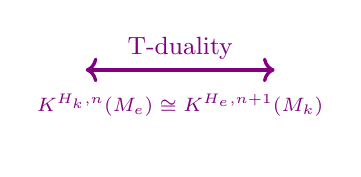
\begin{tikzpicture}[baseline=-1cm]
\draw[<->,very thick,violet] (0,0) -- (2.4,0) node[midway,above,font=\small] {T-duality};
\node[font=\scriptsize,violet] at (1.2,-0.45) {$K^{H_k,n}(M_e)\cong K^{H_e,n+1}(M_k)$};
\end{tikzpicture}
\bundlepic{$M_k\to\Sigma_g$}{flux $e\,[M_k]^\vee$}{green!50!black}
\caption{T-duality for circle bundles over a surface exchanges the Euler number with the number of flux units. Proposition~\ref{prop:tdualcheck} verifies the exchange on the groups of Theorem~\ref{thm:three}.}
\label{fig:tdual}
\end{figure}

\section{Index theory and the Chern character}\label{sec:index}

\subsection{Push-forward and Riemann--Roch}
A D$p$-brane wrapping a submanifold $\iota\colon W\hookrightarrow X$ with Chan--Paton bundle $E\to W$ carries the charge $\iota_!E\in K^*(X)$ \cite{MM97,Wit98}, where $\iota_!$ is the push-forward defined through the Thom isomorphism of the normal bundle $N$ of $W$; this requires $N$ to be K-oriented, that is spin$^c$, which is the Freed--Witten condition in the absence of flux \cite{FW99}. For a complex embedding, with $W$ and $X$ complex manifolds and $N$ the holomorphic normal bundle, the Grothendieck--Riemann--Roch theorem reads
\begin{equation}\label{eq:grr}
\ch(\iota_!E)\,\Td(TX)=\iota_*\bigl(\ch(E)\,\Td(TW)\bigr),\qquad\text{equivalently}\qquad\ch(\iota_!E)=\iota_*\Bigl(\frac{\ch(E)}{\Td(N)}\Bigr),
\end{equation}
since $\iota^*TX=TW\oplus N$ and $\iota_*(\iota^*a\cdot b)=a\cdot\iota_*b$. The denominator is the Todd class of the normal bundle alone; a formula with $\Td(TW)/\Td(N)$ in place of $1/\Td(N)$ fails already for the identity embedding of $\CC P^1$, where it would give $\ch(E)=\ch(E)(1+h)$. For the hyperplane $\CC P^1\subset\CC P^2$ with $E$ trivial the Koszul resolution gives $\iota_!1=1-[\mathcal O(-1)]$, so $\ch(\iota_!1)=1-e^{-h}=h-\tfrac12h^2$, and \eqref{eq:grr} with $\Td(N)=\Td(\mathcal O(1))=1+\tfrac12h$ gives the same, $\iota_*(1-\tfrac12h)=h-\tfrac12h^2$; the incorrect formula gives $h+\tfrac12h^2$. The $-\tfrac12h^2$ is the D0-charge induced on a D2-brane wrapping the line, the gravitational correction to the Wess--Zumino coupling. The general spin$^c$ version of \eqref{eq:grr} replaces Todd classes by the $\Ahat$-genus and the determinant line of the spin$^c$ structure \cite{AS68}.

\subsection{Thom isomorphism}
For a complex vector bundle $V\to X$ of rank $r$ the exterior algebra $\Lambda^\bullet V^*$ pulled back to $V$, with the Koszul differential given by contraction with the tautological section, is exact away from the zero section, and so defines a class $\lambda_V=\sum_k(-1)^k[\Lambda^kV^*]$ in $K^0(D(V),S(V))$; it is a Thom class, and $K^*(X)\to K^*(D(V),S(V))$, $a\mapsto\pi^*a\cdot\lambda_V$, is an isomorphism \cite{Ati67}; the same holds for spin$^c$ real bundles with the spinor Thom class. The push-forward $\iota_!$ is the composition of this isomorphism for $N$ with the map $K^*(D(N),S(N))\to K^*(X)$ induced by a tubular neighbourhood.

\subsection{Chern character and integrality}
The Chern character is a ring isomorphism $K^0(X)\otimes\QQ\to H^{\mathrm{even}}(X;\QQ)$ and an isomorphism $K^1(X)\otimes\QQ\to H^{\mathrm{odd}}(X;\QQ)$ for finite CW complexes, with
\begin{equation}\label{eq:ch}
\ch(E)=r+c_1+\tfrac12(c_1^2-2c_2)+\tfrac16(c_1^3-3c_1c_2+3c_3)+\cdots
\end{equation}
for a bundle of rank $r$ with Chern classes $c_i$. The torsion of $K^*(X)$ is invisible to $\ch$, and it is exactly the torsion that Theorems~\ref{thm:six} and~\ref{thm:three} are about. The Ramond--Ramond field strength of the charge $x\in K^*(X)$ is, in the absence of a B-field,
\begin{equation}\label{eq:rr}
G(x)=\ch(x)\,\sqrt{\Ahat(X)}\in H^*(X;\QQ)
\end{equation}
\cite{MM97,FH00}; with a B-field, that is, a connection on the gerbe with Dixmier--Douady class $H$, given by local two-form potentials whose curvature is a global three-form representing the image of $H$ in real cohomology (for $H$ of infinite order there is no global two-form $B$ with $dB=H$, and a torsion twist carries flat data invisible to the curvature), the Chern character is replaced by the twisted Chern character of $K^{H,*}(X)$ \cite{BM00}; the differential refinement of this picture, with the torsion and the holonomies of the fields and with Calabi--Yau threefolds among the examples, is developed by Grady and Sati \cite{GS22}. The components of $G(x)$ are not integral classes in general: for $x=[\mathcal O(1)]$ on $\CC P^2$ one has $\sqrt{\Ahat}=1-\tfrac1{16}h^2$ and $G(x)=1+h+\tfrac7{16}h^2$. The quantization statement is therefore not that $[G]$ is integral but that $G$ lies in the image of $K^*(X)$ under \eqref{eq:rr}, which is a lattice of full rank in $H^*(X;\QQ)$ different from $H^*(X;\ZZ)$ \cite{FH00}.

\subsection{Torsion charges without flux}
Torsion in $K^*(X)$ also arises without flux. The simplest examples are in Type I, where the charges lie in real K-theory and $\widetilde{KO}(S^{9-p})=KO^{-(9-p)}(\mathrm{pt})$ is $\ZZ/2$ for $p=-1,0,7,8$ \cite{Wit98}; the non-BPS D0-brane of Type I with its $\ZZ/2$ charge is the standard example \cite{Sen98,Wit98}. In Type IIB on a flat space $\RR^8\times S^1$ there is no torsion charge, since $K^1(S^1)\cong\ZZ$ is torsion-free; torsion charges in Type II require either flux, as in Theorems~\ref{thm:six} and~\ref{thm:three}, or torsion in the cohomology of $X$, as for the lens spaces of Table~\ref{tab:three}.

\section{Conclusion}\label{sec:conclusion}

The twisted K-groups of a closed spin$^c$ six-manifold with $H_1=0$ have torsion $C_H=\Tor(H^3/\ZZ H)$ in odd degree and $C_H^\vee$ in even degree, with ranks $b_3-2$ and $2b_2$ for a flux of infinite order; when the cohomology is torsion-free both are $\ZZ/m$, $m$ the divisibility of the flux, and for a Calabi--Yau threefold the ranks are $2h^{2,1}$ and $2h^{1,1}$. The flux removes the D0- and D6-charges and two D3-charges and leaves a D0-charge and a D3-charge of order $m$. When $H^3$ has torsion the torsion component of the flux enters $C_H$, and the manifolds $X_n$ show that fluxes of the same free divisibility can have different charge groups. Three-manifolds behave in the same way, with $K^{H,0}\cong H^2$ and $K^{H,1}\cong H^1\oplus\ZZ/k$, and the groups of circle bundles over surfaces satisfy the exchange predicted by T-duality. Left open are the groups when $H_1(X;\ZZ)\neq0$, where $H^1$ and $H^5$ can be nonzero, $d_3$ has more components and $d_5$ can act; the $K^0(X)$-module structure and the filtration of $K^{H,0}(X)$ beyond the abstract group; and Calabi--Yau examples with torsion in $H^3$, since the manifolds $X_n$ are not K\"ahler.

\section*{Data availability}
The script \texttt{twisted\_k.py} computes every group and identity of this paper from the Betti numbers, torsion and cup products of the spaces, using exact integer and rational arithmetic and Smith normal forms, and runs $45$ checks; it is archived with the LaTeX source of this paper on Zenodo, \doi{10.5281/zenodo.23898720} (release 1.0.0; concept \doi{10.5281/zenodo.23898719}). The computations were set up and run in Python with the assistance of Claude Code.

\section*{Conflicts of interest}
The authors declare no competing interests.

\appendix
\section{The script}\label{app:code}
\texttt{twisted\_k.py} requires Python~3 and SymPy. It computes: the untwisted groups of Table~\ref{tab:kgroups} from the Betti numbers and the K\"unneth theorem; the reduced K-theory of spheres; the Chern character \eqref{eq:ch} of a rank-four bundle on $\CC P^2$; both sides of \eqref{eq:grr} for $\CC P^1\subset\CC P^2$ in $\QQ[h]/(h^3)$ and the failure of the formula with $\Td(TW)/\Td(N)$; the field \eqref{eq:rr} of $\mathcal O(1)$ on $\CC P^2$; the groups of Theorem~\ref{thm:three} for the manifolds of Table~\ref{tab:three}; the exchange of Proposition~\ref{prop:tdualcheck} for $g\le2$ and $0\le e,k\le5$; the groups of Theorem~\ref{thm:six} for the quintic, the bicubic and the Schoen manifold with $m\le3$, with the cokernel and the kernel quotient of Lemma~\ref{lem:lattice} obtained from a unimodular change of basis rather than from the lemma, including a primitive flux with two nonzero coordinates and a flux of divisibility two; the groups of Theorem~\ref{thm:six} with torsion in $H^3$, where $\ker f_H/\ZZ H$ is computed from the lattice and compared with the presentation \eqref{eq:presentation} for $T=\ZZ/2\oplus\ZZ/4$, $\ZZ/2\oplus\ZZ/2\oplus\ZZ/4$, $\ZZ/3\oplus\ZZ/3$ and $\ZZ/2\oplus\ZZ/3\oplus\ZZ/4$, the cyclic formula of Proposition~\ref{prop:presentation} and its splitting criterion for $m\le6$, $n\le8$ and all $t$, the groups of $X_n$ in Corollary~\ref{cor:realized}, and the torsion and zero twists; and the Type I table of $KO^{-n}(\mathrm{pt})$.

{\raggedright
\begin{thebibliography}{99}

\bibitem{AH61}
M.\,F.~Atiyah and F.~Hirzebruch,
\emph{Vector bundles and homogeneous spaces},
Proc.\ Sympos.\ Pure Math.\ \textbf{3} (1961), 7--38.
\doi{10.1090/pspum/003/0139181}

\bibitem{AS68}
M.\,F.~Atiyah and I.\,M.~Singer,
\emph{The index of elliptic operators: I},
Ann.\ of Math.\ (2) \textbf{87} (1968), 484--530.
\doi{10.2307/1970715}

\bibitem{Ati67}
M.\,F.~Atiyah,
\emph{K-theory},
W.\,A.~Benjamin, New York, 1967.

\bibitem{AS04}
M.~Atiyah and G.~Segal,
\emph{Twisted K-theory},
Ukr.\ Mat.\ Visn.\ \textbf{1} (2004), no.~3, 287--330, \href{https://arxiv.org/abs/math/0407054}{arXiv:math/0407054}.

\bibitem{AS06}
M.~Atiyah and G.~Segal,
\emph{Twisted K-theory and cohomology},
in: Inspired by S.\,S.~Chern, Nankai Tracts Math.\ \textbf{11}, World Scientific, Hackensack, 2006, pp.~5--43.
\doi{10.1142/9789812772688_0002}

\bibitem{BB23}
D.~Bhattacharjee, S.\,S.~Roy, R.~Sadhu and A.\,K.~Behera,
\emph{KK theory and K theory for Type II strings formalism},
Asian Res.\ J.\ Math.\ \textbf{19} (2023), no.~9, 79--94.
\doi{10.9734/arjom/2023/v19i9701}

\bibitem{Bha22a}
D.~Bhattacharjee,
\emph{Non-commutativity over canonical suspension $\eta$ for genus $g\ge1$ in hypercomplex structures for potential $\rho_\phi$},
Asian Res.\ J.\ Math.\ \textbf{18} (2022), no.~11, 332--341.
\doi{10.9734/arjom/2022/v18i11607}

\bibitem{BRB22}
D.~Bhattacharjee, S.\,S.~Roy and A.\,K.~Behera,
\emph{Relating Enrique surface with K3 and Kummer through involutions and double covers over finite automorphisms on topological Euler--Poincar\'e characteristics over complex K3 with K\"ahler equivalence},
Research Square (2022).
\doi{10.21203/rs.3.rs-2011341/v1}

\bibitem{BN26}
D.~Bhattacharjee and P.~Nandi,
\emph{Enriques and Kummer surfaces arising from K3 involutions},
Preprints.org (2026).
\doi{10.20944/preprints202602.0098.v1}

\bibitem{BHPV04}
W.\,P.~Barth, K.~Hulek, C.\,A.\,M.~Peters and A.~Van de Ven,
\emph{Compact complex surfaces}, 2nd ed.,
Ergeb.\ Math.\ Grenzgeb.\ (3), vol.~4, Springer, Berlin, 2004.
\doi{10.1007/978-3-642-57739-0}

\bibitem{BM00}
P.~Bouwknegt and V.~Mathai,
\emph{D-branes, B-fields and twisted K-theory},
J.\ High Energy Phys.\ \textbf{03} (2000), 007.
\doi{10.1088/1126-6708/2000/03/007}

\bibitem{BEM04a}
P.~Bouwknegt, J.~Evslin and V.~Mathai,
\emph{T-duality: topology change from H-flux},
Comm.\ Math.\ Phys.\ \textbf{249} (2004), 383--415.
\doi{10.1007/s00220-004-1115-6}

\bibitem{BEM04b}
P.~Bouwknegt, J.~Evslin and V.~Mathai,
\emph{Topology and H-flux of T-dual manifolds},
Phys.\ Rev.\ Lett.\ \textbf{92} (2004), 181601.
\doi{10.1103/PhysRevLett.92.181601}

\bibitem{BHM04}
P.~Bouwknegt, K.~Hannabuss and V.~Mathai,
\emph{T-duality for principal torus bundles},
J.\ High Energy Phys.\ \textbf{03} (2004), 018.
\doi{10.1088/1126-6708/2004/03/018}

\bibitem{CE07}
A.~Collinucci and J.~Evslin,
\emph{Twisted homology},
J.\ High Energy Phys.\ \textbf{03} (2007), 058.
\doi{10.1088/1126-6708/2007/03/058}

\bibitem{DK70}
P.~Donovan and M.~Karoubi,
\emph{Graded Brauer groups and K-theory with local coefficients},
Publ.\ Math.\ Inst.\ Hautes \'Etudes Sci.\ \textbf{38} (1970), 5--25.
\doi{10.1007/BF02684650}

\bibitem{DM07}
C.\,F.~Doran and J.\,W.~Morgan,
\emph{Algebraic topology of Calabi--Yau threefolds in toric varieties},
Geom.\ Topol.\ \textbf{11} (2007), 597--642.
\doi{10.2140/gt.2007.11.597}

\bibitem{FH00}
D.\,S.~Freed and M.\,J.~Hopkins,
\emph{On Ramond--Ramond fields and K-theory},
J.\ High Energy Phys.\ \textbf{05} (2000), 044.
\doi{10.1088/1126-6708/2000/05/044}

\bibitem{FW99}
D.\,S.~Freed and E.~Witten,
\emph{Anomalies in string theory with D-branes},
Asian J.\ Math.\ \textbf{3} (1999), no.~4, 819--852.
\doi{10.4310/AJM.1999.v3.n4.a6}

\bibitem{GS22}
D.~Grady and H.~Sati,
\emph{Ramond--Ramond fields and twisted differential K-theory},
Adv.\ Theor.\ Math.\ Phys.\ \textbf{26} (2022), 1097--1155.
\doi{10.4310/ATMP.2022.v26.n5.a2}

\bibitem{Kap00}
A.~Kapustin,
\emph{D-branes in a topologically nontrivial B-field},
Adv.\ Theor.\ Math.\ Phys.\ \textbf{4} (2000), no.~1, 127--154.
\doi{10.4310/ATMP.2000.v4.n1.a3}

\bibitem{Kas81}
G.\,G.~Kasparov,
\emph{The operator K-functor and extensions of $C^*$-algebras},
Math.\ USSR Izv.\ \textbf{16} (1981), no.~3, 513--572.
\doi{10.1070/IM1981v016n03ABEH001320}

\bibitem{MMS01}
J.~Maldacena, G.~Moore and N.~Seiberg,
\emph{D-brane instantons and K-theory charges},
J.\ High Energy Phys.\ \textbf{11} (2001), 062.
\doi{10.1088/1126-6708/2001/11/062}

\bibitem{MR05}
V.~Mathai and J.~Rosenberg,
\emph{T-duality for torus bundles with H-fluxes via noncommutative topology},
Comm.\ Math.\ Phys.\ \textbf{253} (2005), 705--721.
\doi{10.1007/s00220-004-1159-7}

\bibitem{MM97}
R.~Minasian and G.~Moore,
\emph{K-theory and Ramond--Ramond charge},
J.\ High Energy Phys.\ \textbf{11} (1997), 002.
\doi{10.1088/1126-6708/1997/11/002}

\bibitem{Ros89}
J.~Rosenberg,
\emph{Continuous-trace algebras from the bundle theoretic point of view},
J.\ Austral.\ Math.\ Soc.\ Ser.\ A \textbf{47} (1989), 368--381.
\doi{10.1017/S1446788700033097}

\bibitem{RS87}
J.~Rosenberg and C.~Schochet,
\emph{The K\"unneth theorem and the universal coefficient theorem for Kasparov's generalized K-functor},
Duke Math.\ J.\ \textbf{55} (1987), 431--474.
\doi{10.1215/S0012-7094-87-05524-4}

\bibitem{Sen98}
A.~Sen,
\emph{Stable non-BPS states in string theory},
J.\ High Energy Phys.\ \textbf{06} (1998), 007.
\doi{10.1088/1126-6708/1998/06/007}

\bibitem{Sen98b}
A.~Sen,
\emph{Tachyon condensation on the brane antibrane system},
J.\ High Energy Phys.\ \textbf{08} (1998), 012.
\doi{10.1088/1126-6708/1998/08/012}

\bibitem{Tu09}
J.-L.~Tu,
\emph{Twisted K-theory and Poincar\'e duality},
Trans.\ Amer.\ Math.\ Soc.\ \textbf{361} (2009), 1269--1278.
\doi{10.1090/S0002-9947-08-04706-5}

\bibitem{Wit98}
E.~Witten,
\emph{D-branes and K-theory},
J.\ High Energy Phys.\ \textbf{12} (1998), 019.
\doi{10.1088/1126-6708/1998/12/019}

\end{thebibliography}}

\end{document}
